% Backup slides for the Q&A (not part of the 5-minute pitch), referenced from ../docs/qa_guide.md as B1..B13.
% Numbers: requirements.py, model.py, coverage.py, odd.py, bom.py (CSV files in the repo root).
% Build: latexmk -pdf backup.tex
\documentclass[aspectratio=169,11pt]{beamer}
% Shared look for presentation.tex and backup.tex: quiet ink colors, no theme decoration.
\usetheme{default}
\setbeamertemplate{navigation symbols}{}
\setbeamertemplate{footline}{\hfill\scriptsize\color{gray}\insertframenumber\hspace{1.2em}\vspace{0.6em}}
\setbeamersize{text margin left=0.6cm, text margin right=0.6cm}
\definecolor{ink}{HTML}{0B0B0B}
\definecolor{ink2}{HTML}{52514E}
\definecolor{muted}{HTML}{898781}
\definecolor{good}{HTML}{0A8A0A}
\definecolor{warn}{HTML}{A06E00}
\definecolor{bad}{HTML}{C03030}
\setbeamercolor{frametitle}{fg=ink}
\setbeamercolor{title}{fg=ink}
\setbeamercolor{subtitle}{fg=ink2}
\setbeamercolor{normal text}{fg=ink}
\setbeamercolor{structure}{fg=ink2}
\setbeamerfont{frametitle}{series=\bfseries,size=\large}
\setbeamertemplate{itemize items}{\textbullet}
\usepackage{booktabs}
\usepackage{amsmath}
\usepackage{array}
\newcolumntype{L}[1]{>{\raggedright\arraybackslash}p{#1}}
\graphicspath{{../figures/}}
\newcommand{\smallnote}[1]{{\scriptsize\color{muted}#1}}

\renewcommand{\insertframenumber}{B\arabic{framenumber}}

\begin{document}

% ---------------------------------------------------------------
\begin{frame}{Sensors and their official sources}
  \scriptsize
  \renewcommand{\arraystretch}{1.0}
  \setlength{\tabcolsep}{3pt}
  \begin{tabular}{@{}L{3.2cm} L{7.3cm} L{3.9cm}@{}}
    \toprule
    sensor & numbers we use & source \\
    \midrule
    Innoviz InnovizTwo (Condor) & 120$^\circ$\,$\times$\,28.8$^\circ$; ROI 30$^\circ$\,$\times$\,9.6$^\circ$ at 0.1$^\circ$\,$\times$\,0.05$^\circ$, 210\,m @\,10\,\%
      (90\,\% per pixel, 100\,klx); side FOV 0.2$^\circ$\,$\times$\,0.05$^\circ$, 140\,m @\,10\,\%; 300\,m max; 10\,cm bias; 905\,nm; 20\,FPS
      & datasheet v3.1 (2024) \\
    Hesai OT128 & 360$^\circ$\,$\times$\,40$^\circ$ ($-$25 to +15$^\circ$); 128 channels, each with its own elevation and
      10\,\% range (200\,m on ch.\ 33--64, 30--140\,m on the others, PoD 70\,\%); 0.1$^\circ$ / 0.2$^\circ$ at 10\,Hz;
      0.3--230\,m; $\pm$3\,cm; 3.46\,M pts/s; 29\,W
      & user manual O01-en-260110: 1.6 specifications, appendix A.1 channel table \\
    smartmicro DRVEGRD 171 & 76--77\,GHz; $\pm$50$^\circ$\,$\times$\,$\pm$10$^\circ$; car range 240 / 98 / 42\,m (1.2 / 0.5 / 0.2\,m min);
      range acc.\ 0.6 / 0.25 / 0.1\,m; speed acc.\ 0.07\,m/s; az.\ 0.25$^\circ$; 55\,ms cycle & datasheet 2 Jun 2026 + product sheet \\
    Supertek OX08B40 GMSL2 (H30/H60/H120) & 3840\,$\times$\,2160, 2.1\,$\mu$m, 140\,dB HDR; 30$^\circ$\,$\times$\,16$^\circ$ / 60$^\circ$\,$\times$\,33$^\circ$ /
      120$^\circ$\,$\times$\,66$^\circ$; 30\,FPS & module datasheet + OmniVision brief \\
    SENSING SG3S-ISX031C H190 & 1920\,$\times$\,1536, 3\,$\mu$m, 196$^\circ$\,$\times$\,154$^\circ$, 30\,FPS; 459\,USD listed;
      120\,dB HDR is the Sony ISX031 sensor figure (SENSING only says ``HDR'') & SENSING datasheet (Seeed) \\
    Raytron Horus640-D, 13.5\,mm & 640\,$\times$\,512, 12\,$\mu$m, NETD 35\,mK, 32$^\circ$\,$\times$\,26$^\circ$, 0.8\,mrad, AEC-Q100;
      pedestrian identified at 169\,m (Johnson) & product manual V1.1 (2024) \\
    u-blox ZED-F9K-01A & RTK $<$\,0.2\,m CEP; IMU dead reckoning without GNSS & data sheet UBX-21045820 \\
    \bottomrule
  \end{tabular}

  \vspace{0.4em}
  \smallnote{Every sensor is a specific, buyable product; all numbers above are from its maker's own document.
  Reused on purpose from earlier groups: only the Hesai OT128.}
\end{frame}

% ---------------------------------------------------------------
\begin{frame}{Model: one law per effect (model.py)}
  \footnotesize
  \setlength{\abovedisplayskip}{3pt}\setlength{\belowdisplayskip}{3pt}
  \setlength{\abovedisplayshortskip}{2pt}\setlength{\belowdisplayshortskip}{3pt}
  \begin{columns}[t]
    \column{0.5\textwidth}
    \textbf{Atmosphere}
    \[ \alpha = \frac{3.912}{V}, \qquad \alpha_\text{rain} = 0.365\,R^{0.63}\,\text{km}^{-1} \]
    \smallnote{Koschmieder, fog and snow, same at 550 and 905\,nm (Kim 2001); rain $R$ in mm/h}\par\medskip
    \textbf{Lidar} (Exercise 3 model)
    \[ p = 1 - \exp\!\Big(-c\,\frac{\rho}{R^2}\,e^{-2\alpha R}\Big), \quad p(R_{10\%}, 10\,\%) = p_0 \]
    detected if $P(K \ge 5) \ge 99\,\%$, $K \sim \mathrm{Bin}(n, p)$, $n$ = beams on the target
    (grid offset: $n$ rounds up or down)
    \smallnote{InnovizTwo: $p_0$ = 0.9 (datasheet). OT128: $K$ sums the channels that hit the target from 1.75\,m,
    each with its own $R_{10\%}$, $p_0$ = 0.7 (manual A.1)}\par\medskip

    \textbf{Radar}
    \[ R^4\, 10^{2\gamma R/10} = R_0^4\, g(\varphi)^4\, \frac{\sigma}{\sigma_\text{car}} \]
    \smallnote{$\gamma = 1.02\,R_\text{rain}^{0.73}$\,dB/km (ITU-R P.838-3, 77\,GHz); $g(\varphi)$ from a one-way gain of
    $-3(\varphi/40^\circ)^2$\,dB}
    \column{0.5\textwidth}
    \textbf{Camera}
    \[ R = \min\Big(\frac{H}{25\,\mathrm{IFOV}},\; \frac{1}{\alpha}\ln\frac{C_0}{0.05\,(1+G)},\; \sqrt{I/E_\text{min}}\Big) \]
    25\,px object height (KITTI); contrast $\ge 0.05$; glare $G$; at night the low beam
    ($I$ = 4000\,cd, $E_\text{min}$ = 1\,lux) lights pedestrians only; HDR deficit costs $10^{-\Delta\text{dB}/20}$\par\medskip

    \textbf{Thermal}
    \[ R = \min\Big(\frac{H}{25\,\mathrm{IFOV}},\; -\frac{1}{\alpha_\text{LWIR}}\ln\frac{5\,\mathrm{NETD}}{\Delta T}\Big) \]
    \smallnote{$\alpha_\text{LWIR}$ = 0.4\,$\times$ visible in fog (assumption, see B10)}\par\medskip

    \textbf{Stopping distance and safe speed}
    \[ d = v\,t_r + \frac{v^2}{2a}, \quad v_\text{safe} = a\Big(-t_r + \sqrt{t_r^2 + 2d/a}\Big) \]
    \smallnote{$t_r$ = 1\,s, $a$ = 3\,m/s$^2$; $d$ = range of the 2nd-best modality}
  \end{columns}
\end{frame}

% ---------------------------------------------------------------
\begin{frame}{Detection range per sensor and condition (ranges.csv)}
  \centering\scriptsize
  \renewcommand{\arraystretch}{1.15}
  \setlength{\tabcolsep}{2.5pt}
  \begin{tabular}{@{}lrrrrrrr@{}}
    \toprule
    pedestrian / car [m] & clear & night & fog 200\,m & rain 25\,mm/h & snow & low sun & tunnel exit \\
    \midrule
    InnovizTwo lidar & 231 / 300 & 231 / 300 & 98 / 114 & 178 / 240 & 150 / 197 & 231 / 300 & 231 / 300 \\
    Hesai OT128 lidar & 160 / 214 & 160 / 214 & 80 / 92 & 136 / 176 & 114 / 147 & 160 / 214 & 160 / 214 \\
    smartmicro DRVEGRD 171 radar & 100 / 240 & 100 / 240 & 100 / 239 & 89 / 190 & 98 / 234 & 100 / 240 & 100 / 240 \\
    Supertek OX08B40 30$^\circ$ & 557 / 464 & \textbf{63} / 464 & 92 / 106 & 557 / 464 & 458 / 464 & 557 / 464 & 557 / 464 \\
    Supertek OX08B40 60$^\circ$ & 270 / 225 & \textbf{63} / 225 & 92 / 106 & 270 / 225 & 270 / 225 & 270 / 225 & 270 / 225 \\
    Supertek OX08B40 120$^\circ$ & 135 / 113 & \textbf{63} / 113 & 92 / 106 & 135 / 113 & 135 / 113 & 135 / 113 & 135 / 113 \\
    SENSING ISX031 fisheye & 41 / 34 & 41 / 34 & 41 / 34 & 41 / 34 & 41 / 34 & 41 / 34 & 41 / 34 \\
    Raytron Horus640-D LWIR & 90 / 75 & 90 / 75 & 90 / 75 & 90 / 75 & 90 / 75 & 90 / 75 & 90 / 75 \\
    \bottomrule
  \end{tabular}

  \vspace{0.6em}
  \raggedright
  \begin{itemize}
    \item Night: a camera sees a pedestrian only as far as the low beam lights it (63\,m); cars carry their own lights.
    \item InnovizTwo 231\,m vs.\ 235\,m in Exercise 3: here clear air has 23\,km visibility instead of none.
    \item Thermal: 90\,m by our 25\,px rule; Raytron's 169\,m uses the looser Johnson identification criterion.
    \item Glare and the tunnel exit cost contrast, not range, in clear air: 140\,dB HDR covers a 125\,dB scene.
  \end{itemize}
\end{frame}

% ---------------------------------------------------------------
\begin{frame}{How each spider axis is scored (model.py, sensor\_scores)}
  \footnotesize
  \renewcommand{\arraystretch}{1.2}
  \begin{tabular}{@{}L{2.7cm} L{8.2cm} L{3.0cm}@{}}
    \toprule
    axis & score (0..1) & kind \\
    \midrule
    Contrast, resolution & pixels / points / radar cells on a pedestrian at 50\,m, log scale 1 $\to$ 1000, $\times$ signal left & physics \\
    Range & car detection range / 253\,m & physics \\
    Color & camera 1, lidar 0.15 (NIR intensity), thermal and radar 0; $\times$ signal left; camera $\times$0.3 at night & \textbf{rule} \\
    Speed detection & radial-speed error known within 100\,ms, log 5 $\to$ 0.05\,m/s: radar Doppler, lidar two ranges,
      camera/thermal image-height change (1\,px noise) & physics \\
    3D reconstruction & mean of depth error at 50\,m (log 5\,m $\to$ 2\,cm) and the resolution score & physics \\
    Living objects & cap (thermal 1, camera 0.85, lidar 0.7, radar 0.3) $\times$ signal left $\times$ min(1, pedestrian range / 50\,m) & cap is a \textbf{rule} \\
    \bottomrule
  \end{tabular}

  \vspace{0.6em}
  \begin{itemize}
    \item \emph{Signal left}: the share of the clear-day signal at 50\,m in this condition (lidar return probability,
      radar attenuation, camera contrast incl.\ low-beam light, thermal $\Delta T\,e^{-\alpha R}$).
    \item A modality's polygon is its best forward-looking sensor; a condition group takes the worst sub-case.
    \item Whole suite = best modality per axis.
  \end{itemize}
\end{frame}

% ---------------------------------------------------------------
\begin{frame}{Requirements in detail (requirements.py)}
  \begin{columns}[c]
    \column{0.45\textwidth}
    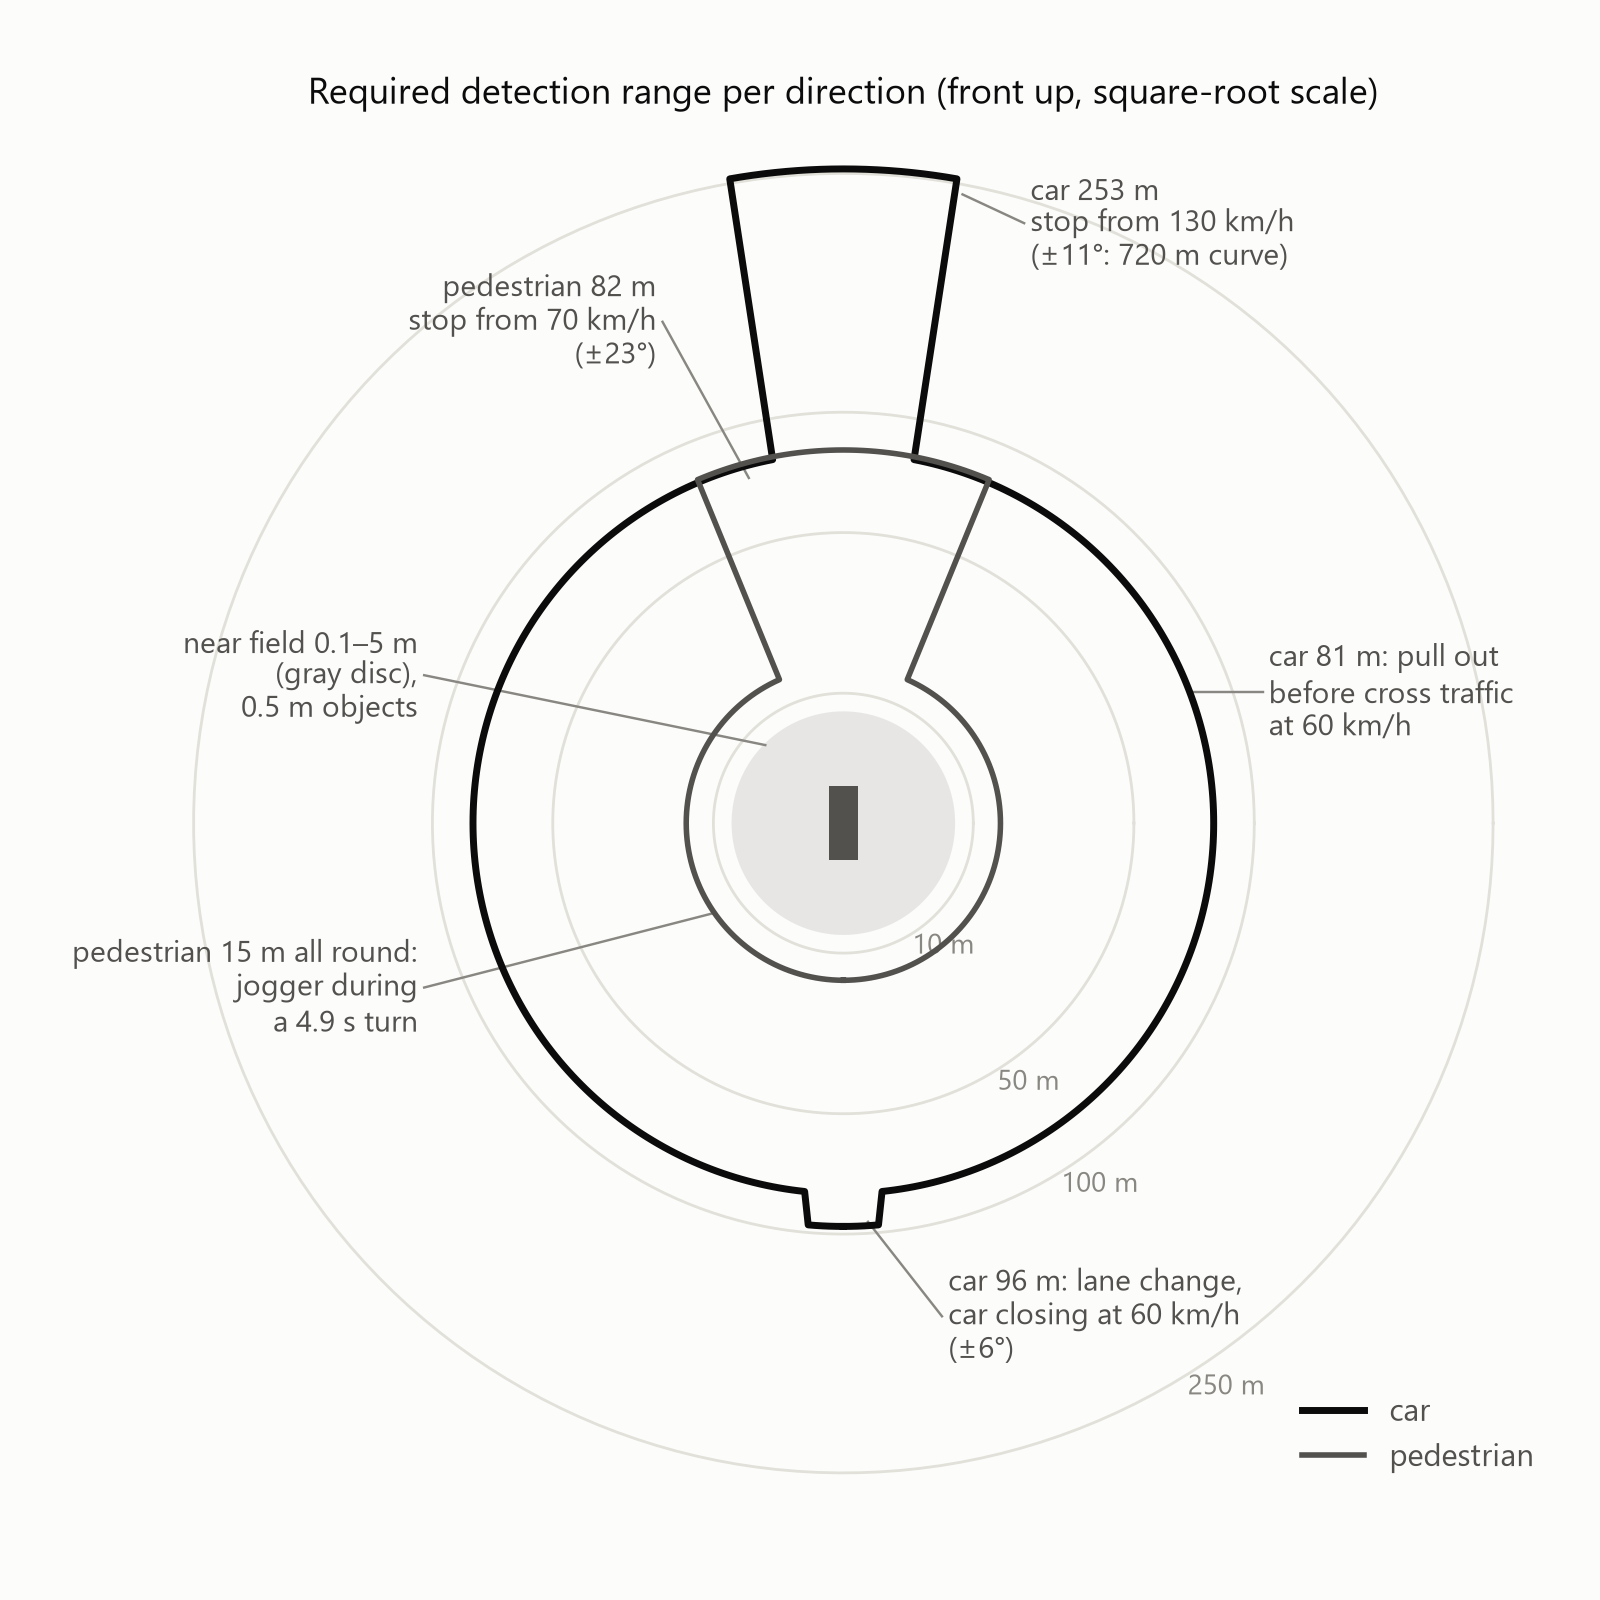
\includegraphics[width=\textwidth]{requirements_detail.png}
    \column{0.53\textwidth}
    \footnotesize
    \begin{itemize}
      \item $t_r$ = 1\,s detection to action, $a$ = 3\,m/s$^2$ comfortable braking.
        With the Exercise 3 emergency values (0.5\,s, 6\,m/s$^2$) 130\,km/h needs only 127\,m.
      \item Front cone: a lane on a 720\,m curve is $d/(2R_c)$ off-axis at $d$ = 253\,m (10$^\circ$), plus a
        3.5\,m lane offset: $\pm$11$^\circ$. Pedestrians: 120\,m urban curve, 5\,m kerb offset: $\pm$23$^\circ$.
      \item Sides: clearing two lanes from a stop takes $1\,\mathrm{s} + \sqrt{2\cdot15\,\mathrm{m}/2\,\mathrm{m/s^2}}$ = 4.9\,s;
        cross traffic at 60\,km/h covers 81\,m.
      \item Rear: 3\,s lane change with a car 60\,km/h faster, which then brakes at 3\,m/s$^2$: 50 + 46 = 96\,m ($\pm$6$^\circ$).
      \item Pedestrians around: a jogger at 3\,m/s during the 4.9\,s: 15\,m.
      \item Near field: 0.1--5\,m from the body, objects 0.5\,m tall (kerb, bollard, crouching child).
    \end{itemize}
  \end{columns}
\end{frame}

% ---------------------------------------------------------------
\begin{frame}{Mounting positions}
  \begin{columns}[c]
    \column{0.50\textwidth}
    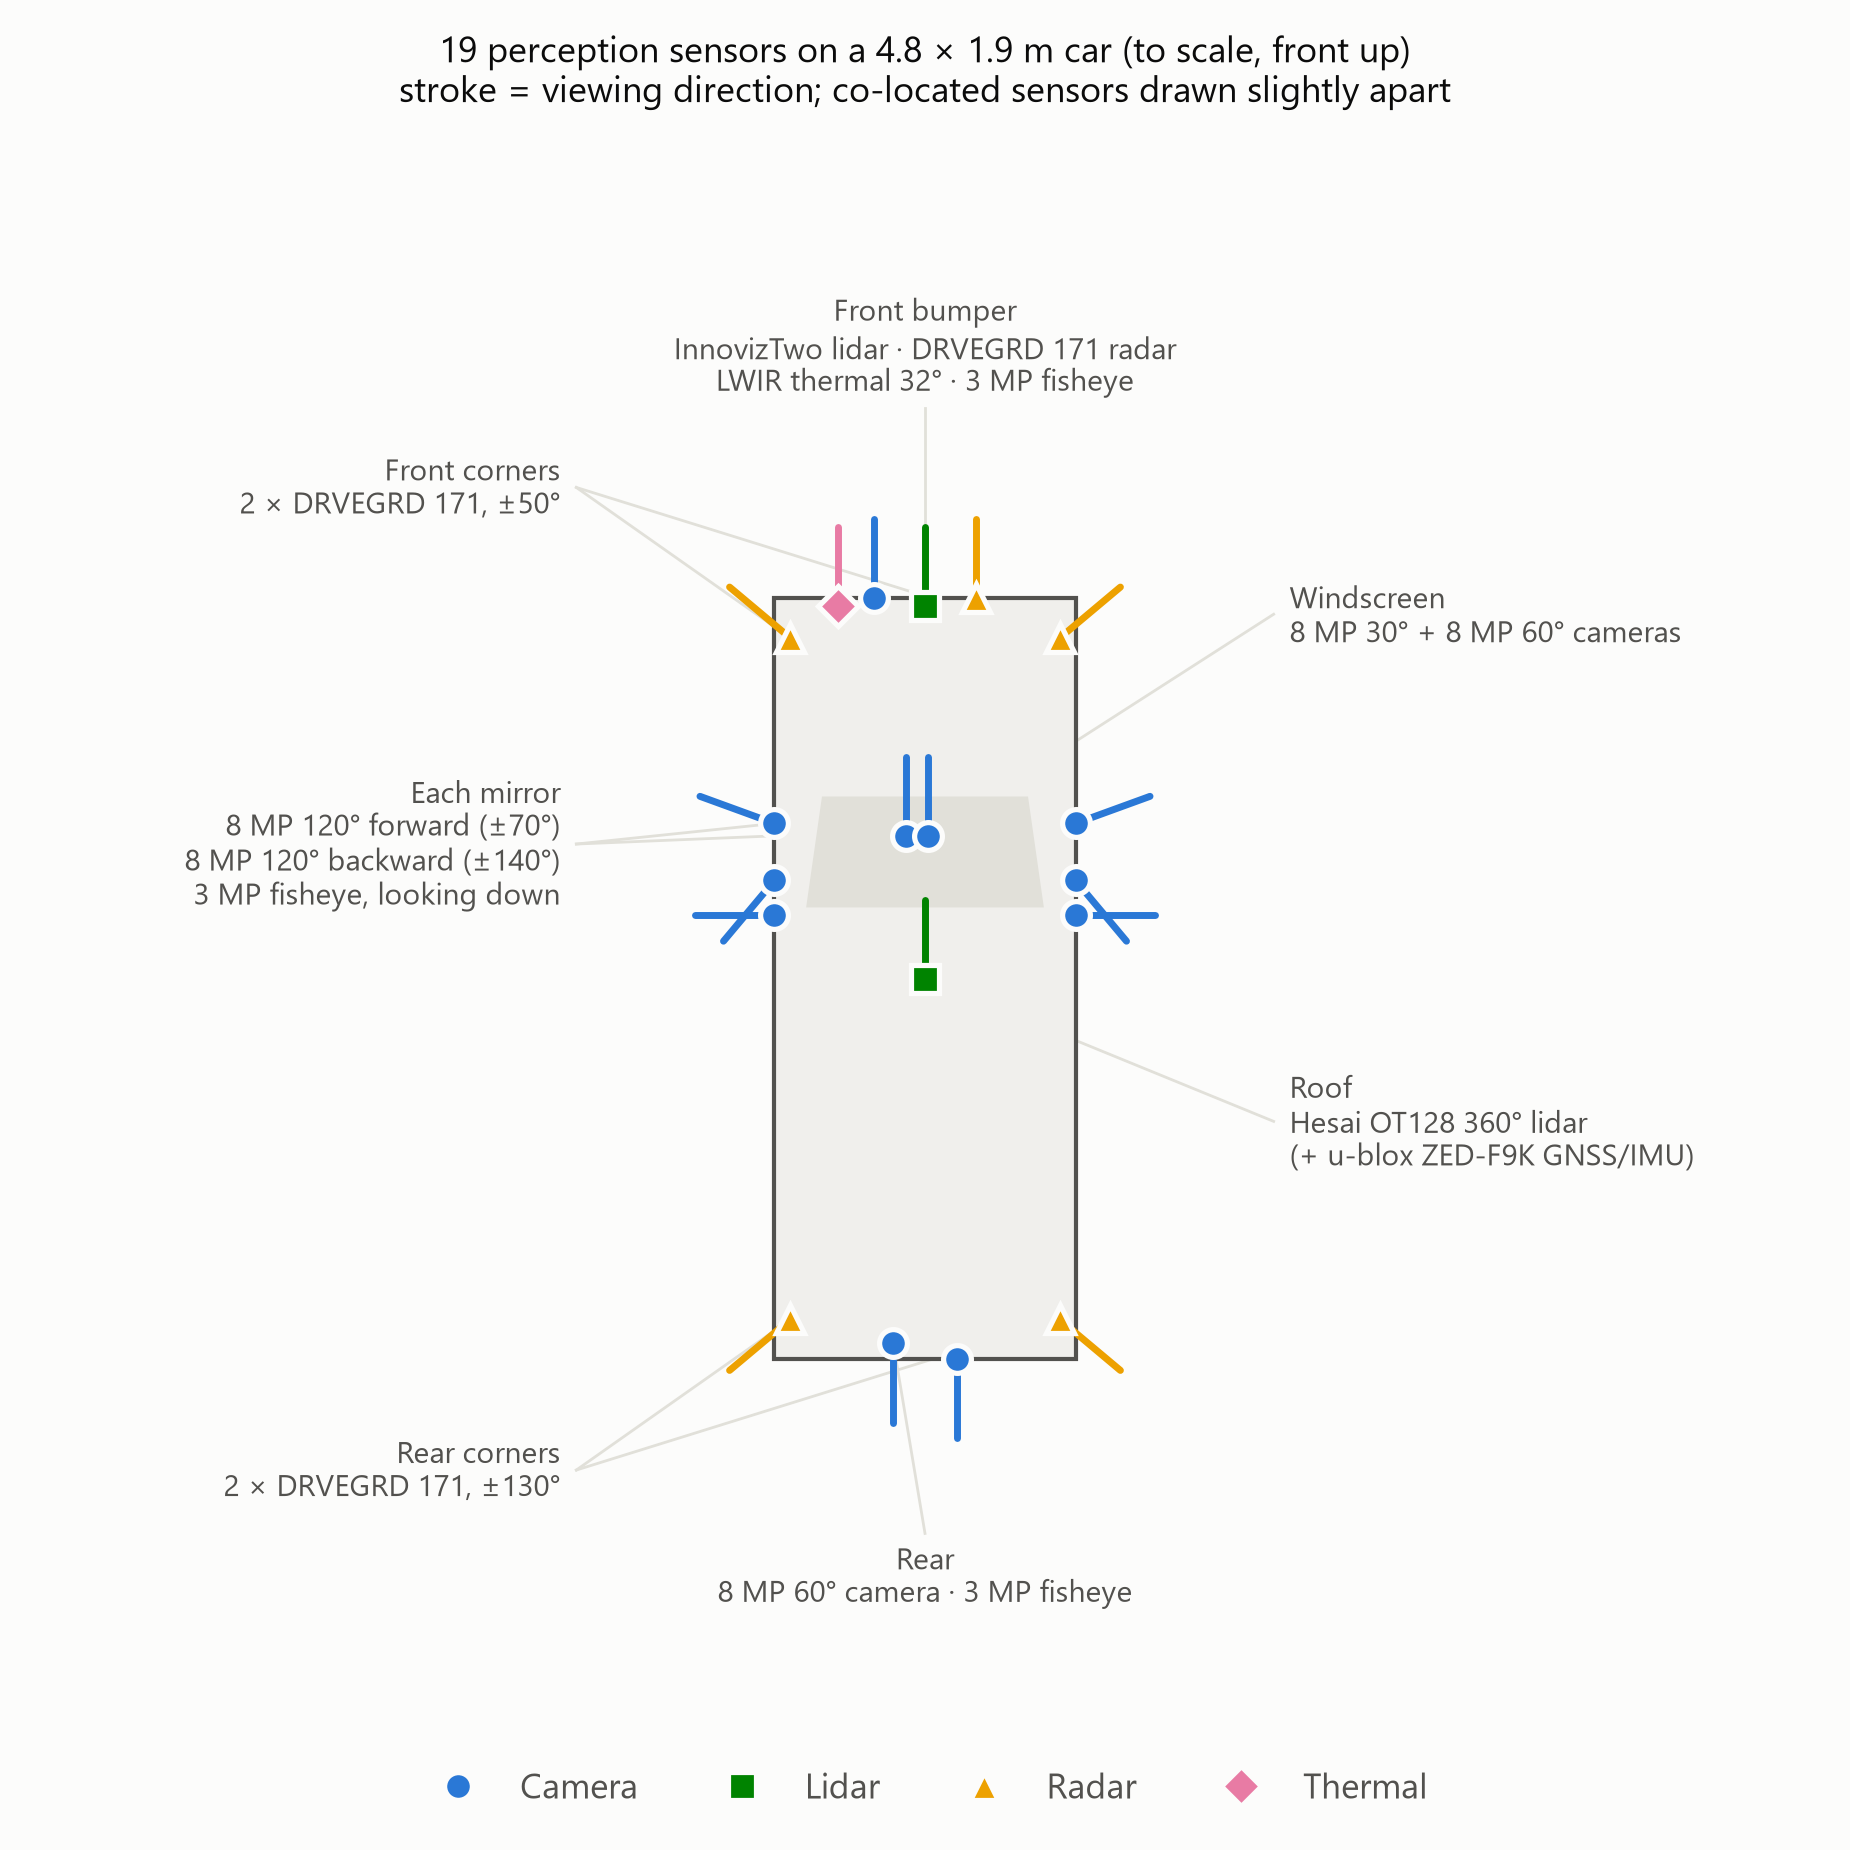
\includegraphics[width=\textwidth]{suite_layout_detail.png}
    \column{0.48\textwidth}
    \footnotesize
    \begin{itemize}
      \item Front lidar low in the bumper (0.6\,m): its ROI looks along the road; the roof lidar (1.75\,m) sees over cars.
      \item Radars: front + four corners at $\pm$50$^\circ$ and $\pm$130$^\circ$, each $\pm$50$^\circ$; they overlap at the sides.
        Every radar alternates extra-long-range (240\,m) and short-range (0.2--42\,m) cycles.
      \item Mirror cameras: 120$^\circ$ forward ($\pm$70$^\circ$) and backward ($\pm$140$^\circ$) cover the sides and the
        adjacent lanes; the 3\,MP fisheyes look down for the near field.
      \item Thermal next to the front lidar: the night-pedestrian case is ahead.
      \item RTK GNSS/IMU at the centre, with an HD map for lane-level position.
    \end{itemize}
  \end{columns}
\end{frame}

% ---------------------------------------------------------------
\begin{frame}{What each modality reaches (clear day, car target)}
  \centering
  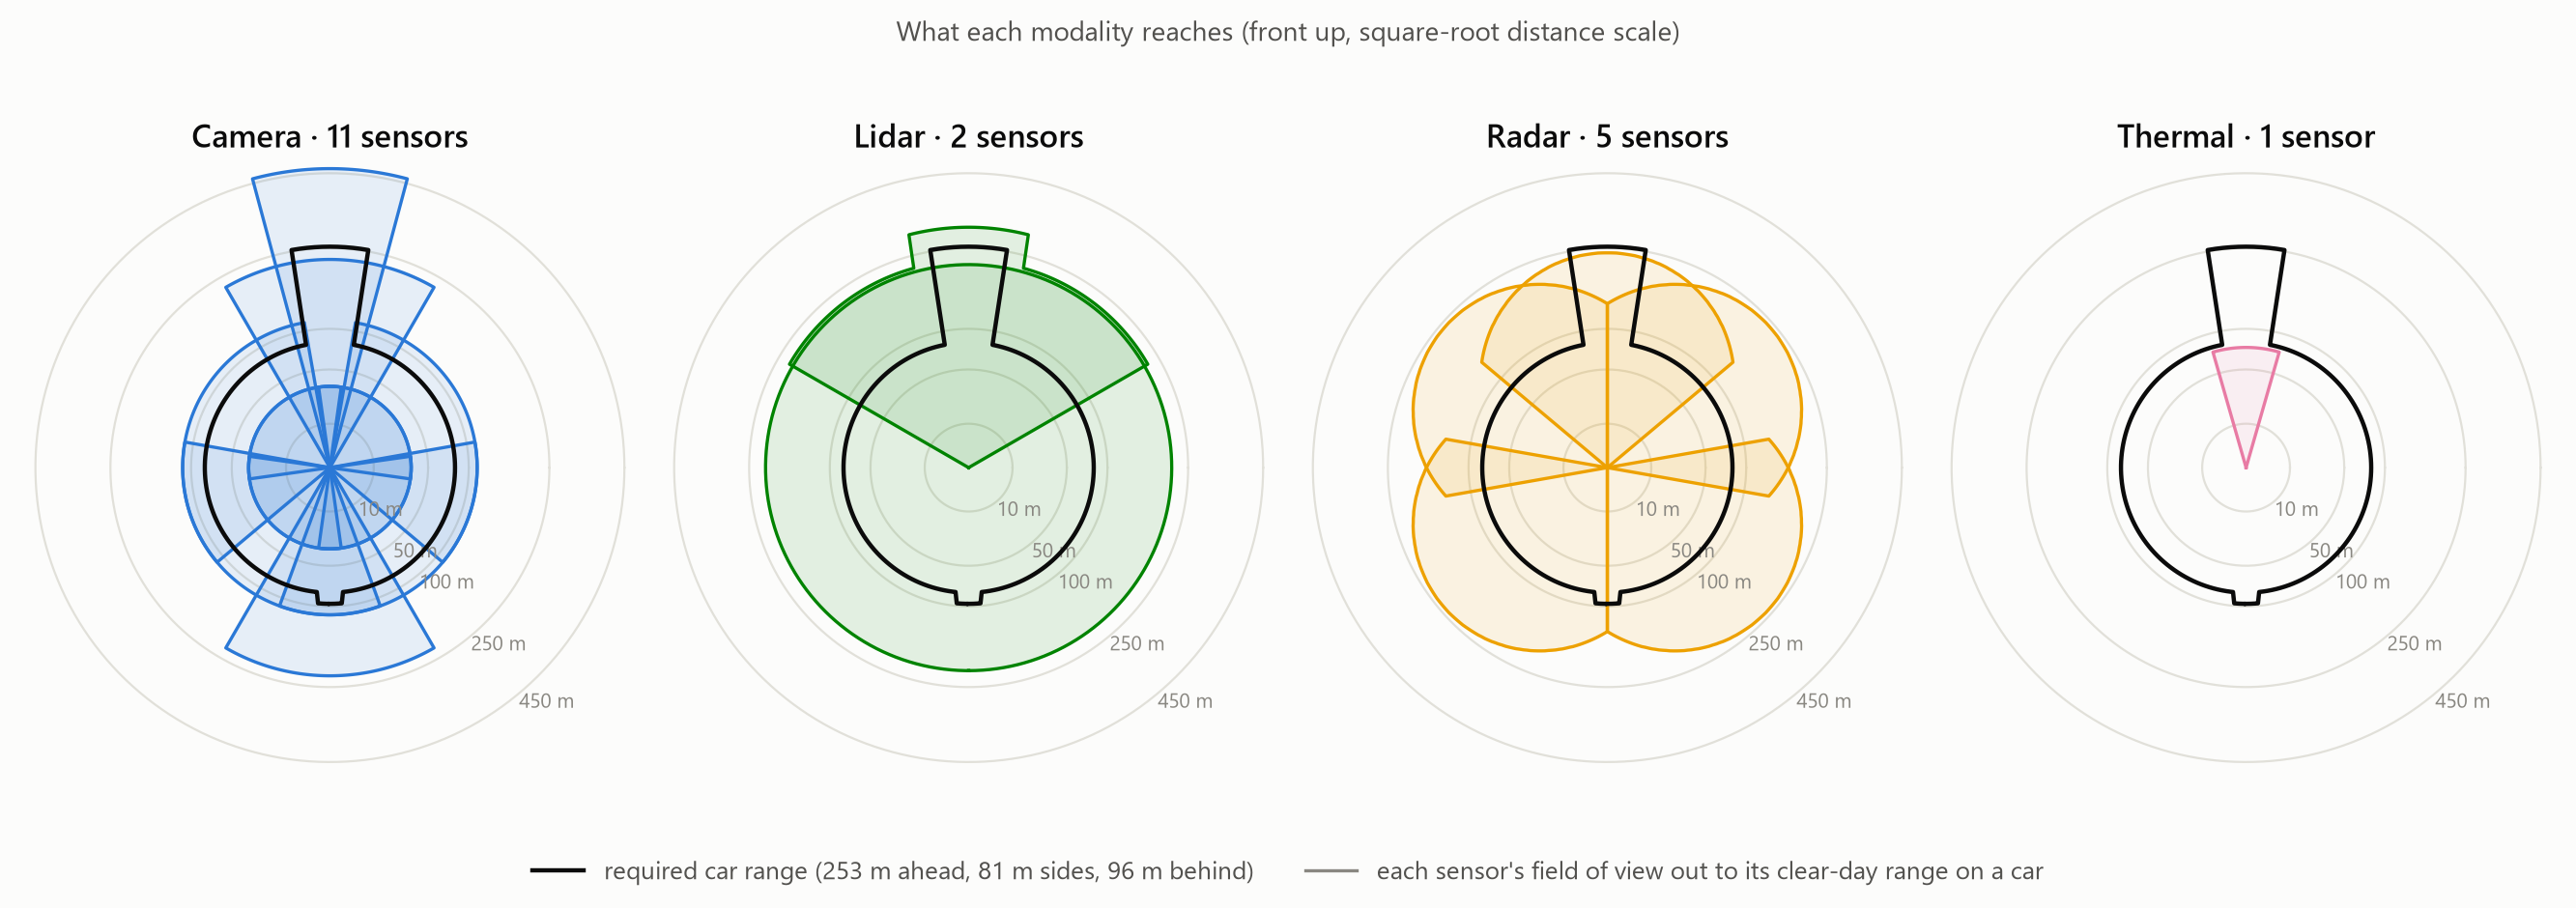
\includegraphics[width=\textwidth]{reach_by_modality.png}

  \footnotesize\raggedright
  Black: required car range. Radar wedges shrink off boresight (antenna pattern); the InnovizTwo wedge steps down
  outside its 30$^\circ$ ROI (140\,m @\,10\,\%). Thermal (75\,m on a car) never reaches the 81\,m side requirement:
  it is there for pedestrians ahead.
\end{frame}

% ---------------------------------------------------------------
\begin{frame}{Coverage in detail (1/2): which modality reaches the required range}
  \centering
  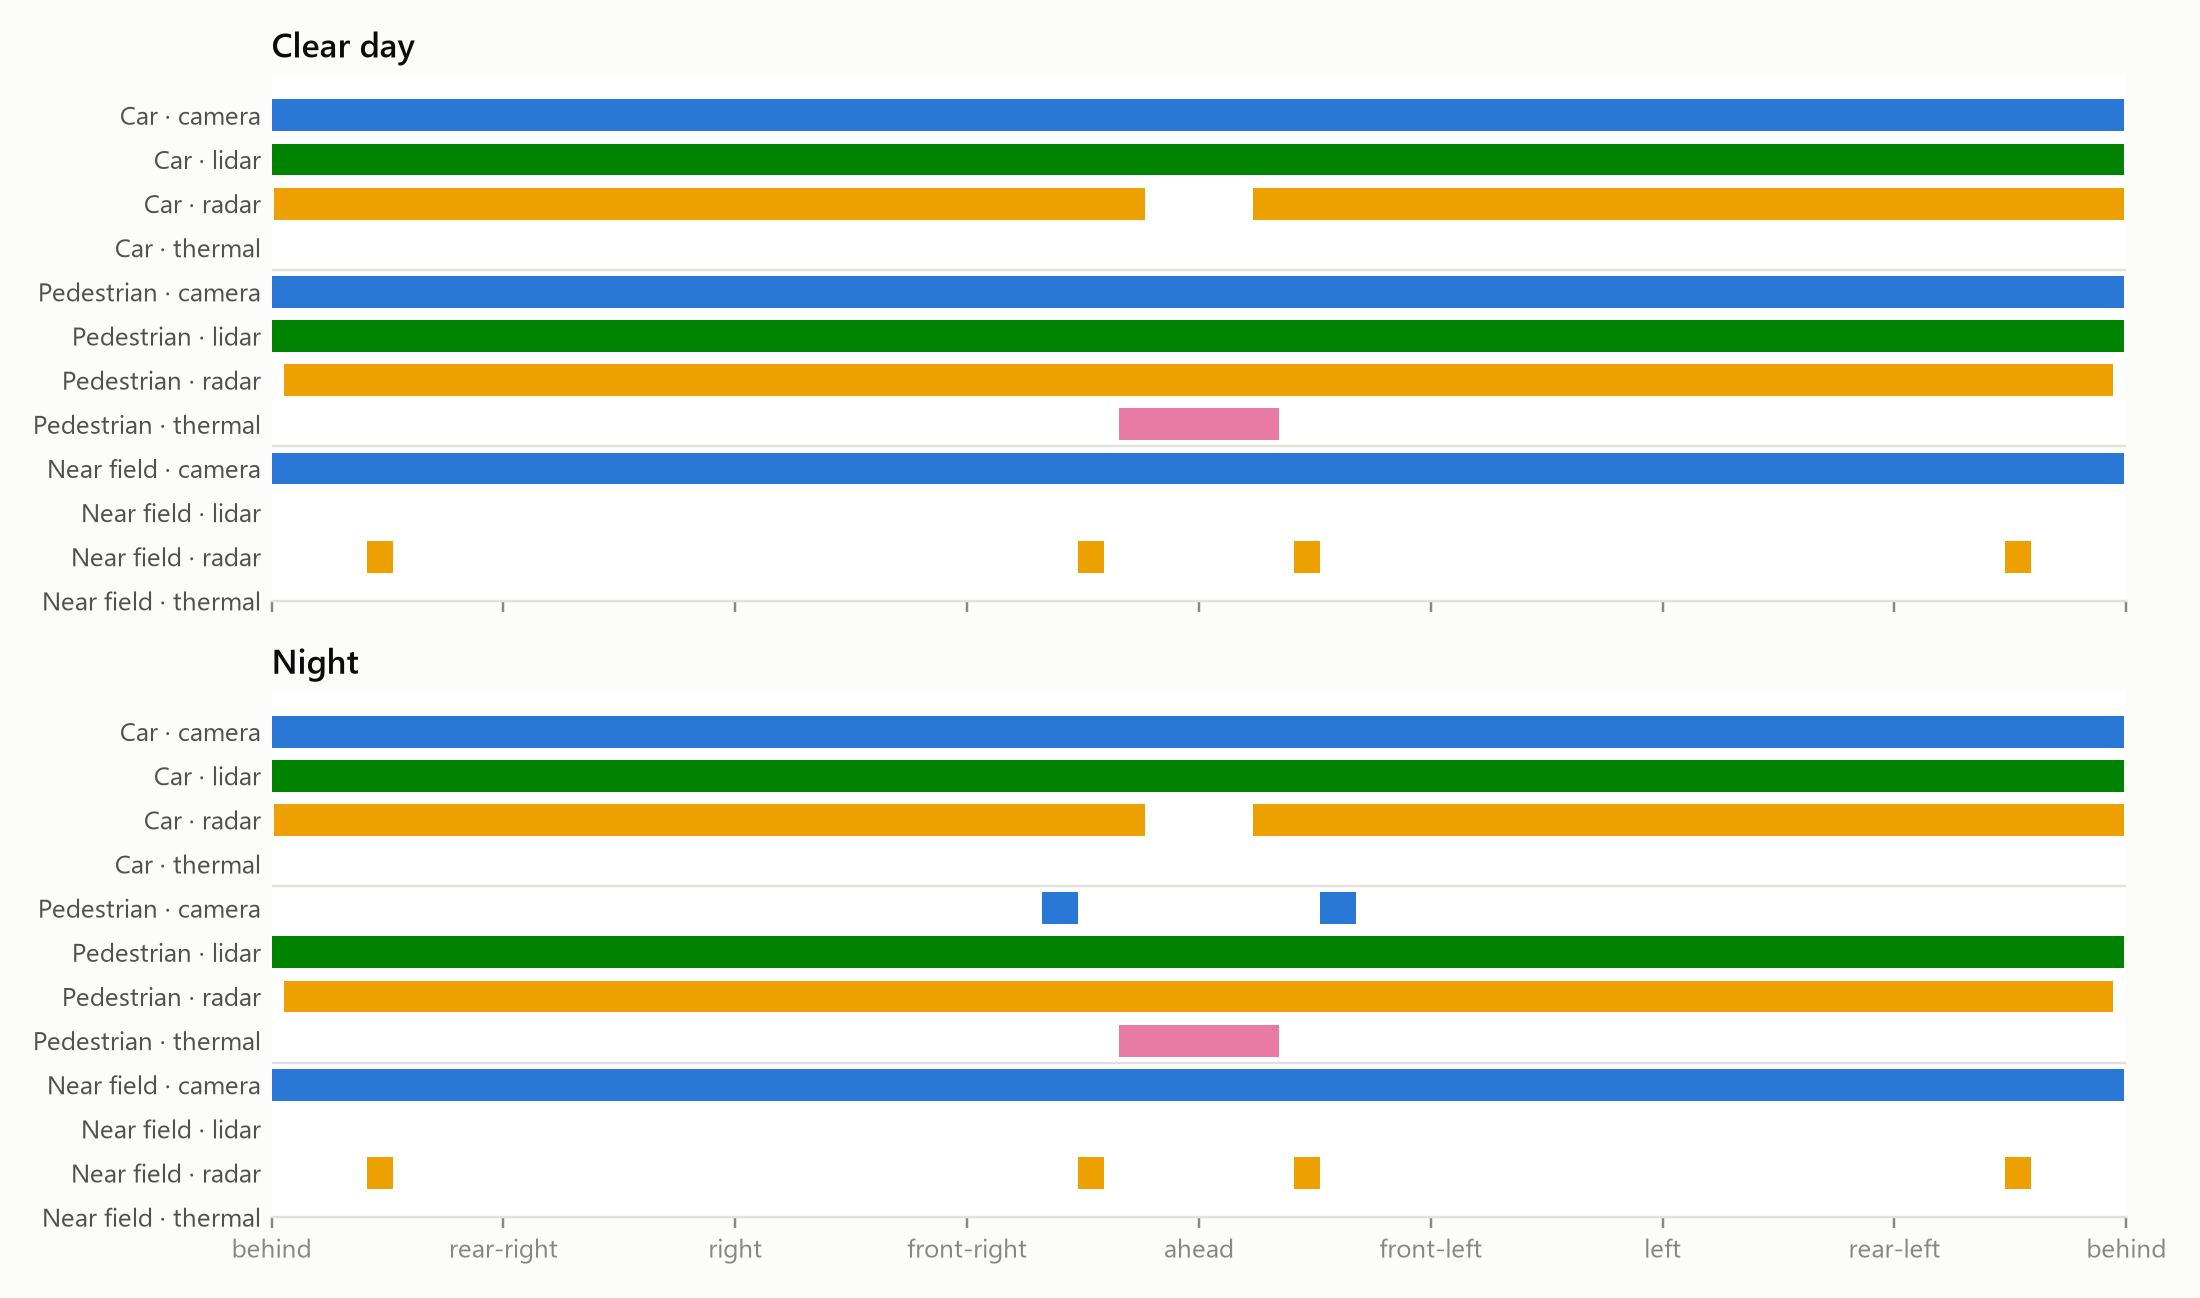
\includegraphics[height=0.86\textheight]{coverage_detail_1.png}
\end{frame}

\begin{frame}{Coverage in detail (2/2): worst sub-case of each condition}
  \centering
  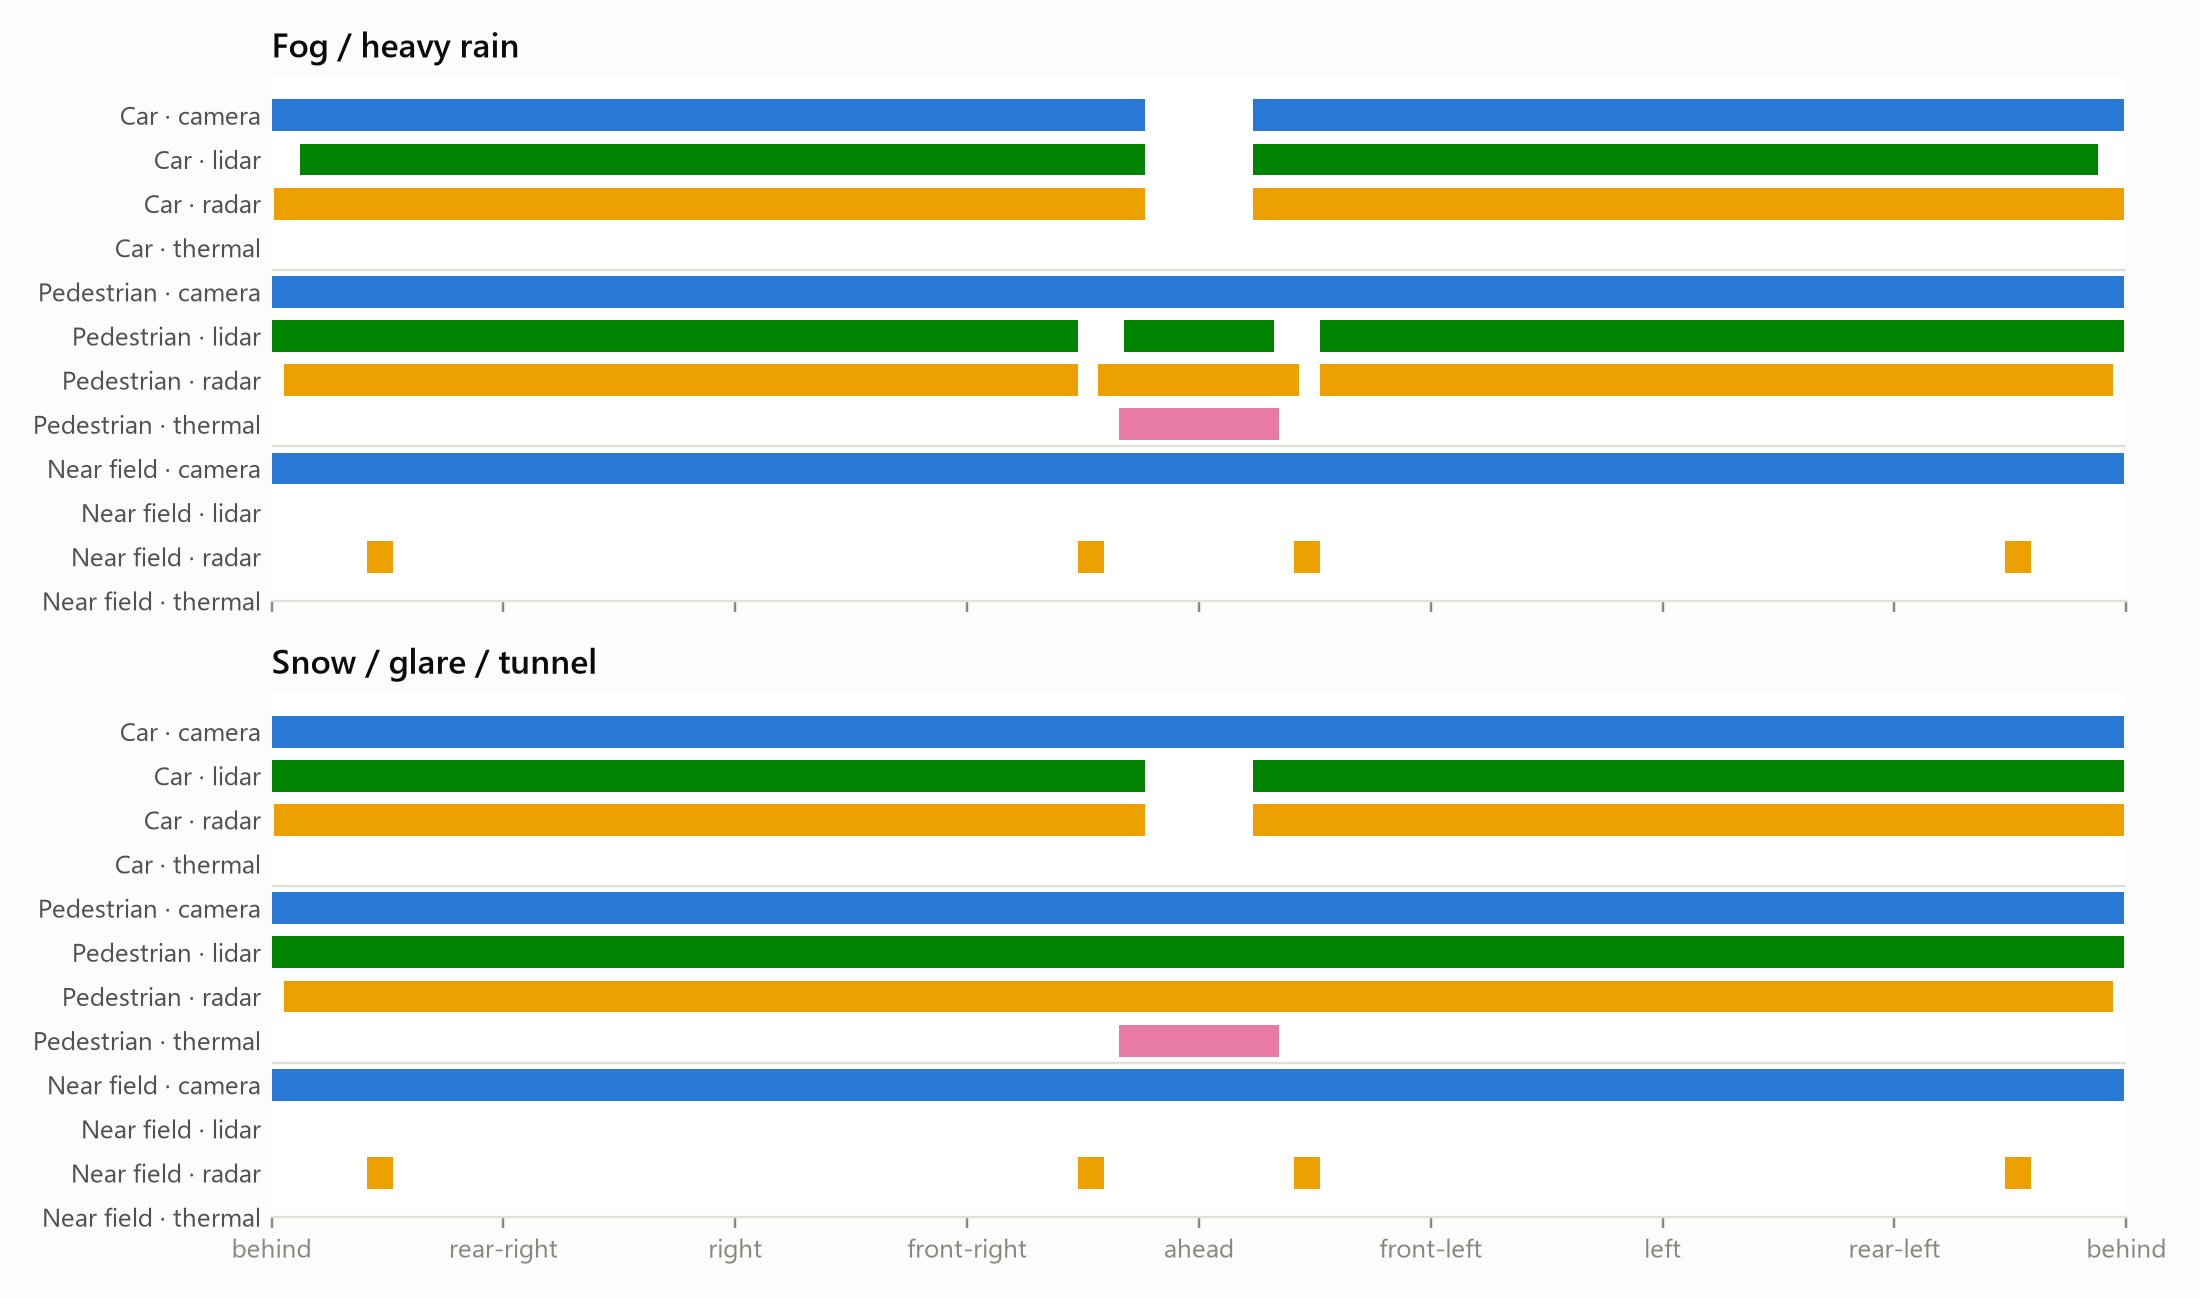
\includegraphics[height=0.80\textheight]{coverage_detail_2.png}

  \scriptsize\color{muted}
  coverage.csv lists every bearing, condition and ring.
\end{frame}

% ---------------------------------------------------------------
\begin{frame}{Safe speed per condition (odd.py, safe\_speed.csv)}
  \footnotesize
  \centering
  \renewcommand{\arraystretch}{1.12}
  \begin{tabular}{@{}llrrrrrrr@{}}
    \toprule
    condition & target & camera & lidar & radar & thermal & 2nd best & v, 2 mod. & v, best \\
    \midrule
    clear day & car & 464 & 300 & 240 & 75 & 300\,m & 142 & 179 \\
     & pedestrian & 557 & 231 & 100 & 90 & 231\,m & 124 & 198 \\
    night & car & 464 & 300 & 240 & 75 & 300\,m & 142 & 179 \\
     & pedestrian & 63 & 231 & 100 & 90 & 100\,m & \textbf{78} & 124 \\
    fog 200\,m & car & 106 & 114 & 239 & 75 & 114\,m & \textbf{84} & 126 \\
     & pedestrian & 92 & 98 & 100 & 90 & 98\,m & \textbf{77} & 78 \\
    snow & car & 464 & 197 & 234 & 75 & 234\,m & 124 & 179 \\
     & pedestrian & 458 & 150 & 98 & 90 & 150\,m & 98 & 178 \\
    \bottomrule
  \end{tabular}

  \vspace{0.6em}
  \raggedright
  \begin{itemize}
    \item Ranges straight ahead in metres; speeds in km/h; worst sub-case of each group (rain is milder than fog).
    \item Fog sweep (car): 84\,km/h at 200\,m visibility, 66--67\,km/h at 50--100\,m, 43--66\,km/h at 20--50\,m.
      If LWIR sees no further than visible light in fog: 52--67 and 35--52\,km/h (our 0.4 ratio is the main uncertainty).
    \item Radar alone would allow 126\,km/h in fog, but nothing confirms what it sees.
  \end{itemize}
\end{frame}

% ---------------------------------------------------------------
\begin{frame}{Our assumptions and the model's limits}
  \scriptsize
  \begin{columns}[t]
    \column{0.5\textwidth}
    \textbf{Assumptions (not from datasheets)}
    \begin{itemize}
      \item Lidar: $\ge$5 returns with 99\,\%; flat road (OT128 channels hit the target by geometry)
      \item Camera: 25\,px, contrast 0.05, pedestrian 0.3, car 0.4; glare $G$ = 3; tunnel exit 125\,dB
      \item Night: unlit road; low beam 4000\,cd, $\pm$30$^\circ$, 1\,lux needed
      \item Weather: clear 23\,km, fog 200\,m, snow 1\,km + 50\,\% lidar clutter, rain 25\,mm/h
      \item LWIR fog extinction 0.4\,$\times$ visible (literature 0.2--1); $\Delta T$ 3--15\,K
      \item Radar: pedestrian 0.3\,m$^2$, car 10\,m$^2$; 3\,dB half-width 40$^\circ$; interleaved modes
      \item Requirements: $t_r$ = 1\,s, $a$ = 3\,m/s$^2$, curve radii, jogger 3\,m/s
      \item Color and living-object caps are rules
    \end{itemize}
    \column{0.5\textwidth}
    \textbf{Not modelled}
    \begin{itemize}
      \item Dirt, spray, snow or ice on a sensor (total blockage)
      \item Raindrops on lenses (rain hurts the camera only through the air here)
      \item False positives, multipath, interference between radars or lidars
      \item Occlusion by other road users; terrain and crests
      \item Classification quality beyond the detection rules
      \item Compute, latency jitter and sensor failure rates
    \end{itemize}
    \vspace{0.4em}
    \textbf{Sensitivity that changes a conclusion}
    \begin{itemize}
      \item LWIR ratio 0.4 $\to$ 1.0: at 50\,m visibility the safe speed drops from 66 to 52\,km/h (car)
      \item Radar reaches 240\,m, 5\,\% short of 253\,m (6\,\% in fog, 8\,\% in snow): a slightly longer-range
        radar would be the 2nd modality ahead in both
    \end{itemize}
  \end{columns}
\end{frame}

% ---------------------------------------------------------------
\begin{frame}{Cost (bom.py)}
  \centering\footnotesize
  \renewcommand{\arraystretch}{1.12}
  \begin{tabular}{@{}llrrr@{}}
    \toprule
    modality & model & count & unit [USD] & subtotal \\
    \midrule
    lidar & Innoviz InnovizTwo & 1 & 1,000 est. & 1,000 \\
    lidar & Hesai OT128 & 1 & 3,000 est. & 3,000 \\
    radar & smartmicro DRVEGRD 171 & 5 & 400 est. & 2,000 \\
    camera & Supertek OX08B40 GMSL2, 30$^\circ$ / 60$^\circ$ / 120$^\circ$ & 1 + 2 + 4 & 300 est. & 2,100 \\
    camera & SENSING ISX031 fisheye & 4 & 459 listed & 1,836 \\
    thermal & Raytron Horus640-D & 1 & 800 est. & 800 \\
    GNSS/IMU & u-blox ZED-F9K & 1 & 250 est. & 250 \\
    \midrule
    & \textbf{total} & \textbf{20} & & \textbf{10,986} \\
    \bottomrule
  \end{tabular}

  \vspace{0.6em}
  \raggedright
  No cost target. Sensors only: no compute, cleaning, wiring or calibration. Volume prices for lidar are falling fast;
  the estimates are order-of-magnitude.
\end{frame}

% ---------------------------------------------------------------
\begin{frame}{Closing the gaps: what we would add next}
  \footnotesize
  \renewcommand{\arraystretch}{1.2}
  \begin{tabular}{@{}L{3.4cm} L{5.8cm} L{4.6cm}@{}}
    \toprule
    gap (from our coverage map) & why & fix \\
    \midrule
    Near field: cameras alone on 340$^\circ$ & lidar/radar minimum range 0.2--0.3\,m; nothing looks down beside the doors &
      a ring of 12 ultrasonic parking sensors (they reach a few metres), a few USD each \\
    Fog / snow ahead: $<$\,2 modalities at 253\,m & radar 239\,m is 6\,\% short; optical sensors halve &
      longer-range imaging radar, or slow down (84\,km/h at 200\,m fog) \\
    Straight behind: lidar only at night (5$^\circ$), camera only in fog (1$^\circ$) & corner radars end at $\pm$50$^\circ$ off their
      axis; unlit at night; OT128 reaches 92\,m in fog, 96\,m needed & a rear radar (or a rear thermal camera) \\
    Blocked sensors & snow, ice, spray &
      cleaning (washers, heaters) + detect blockage + safe stop \\
    \bottomrule
  \end{tabular}
\end{frame}

\end{document}
